\documentclass[11pt,a4paper]{article}
\usepackage[T1]{fontenc}
\usepackage{lmodern}
\usepackage[margin=22mm]{geometry}
\usepackage{graphicx,booktabs,amsmath,array}
\usepackage{hyperref}
\usepackage[numbers]{natbib}
\graphicspath{{figures/}}
\renewcommand{\thetable}{S\arabic{table}}
\renewcommand{\thefigure}{S\arabic{figure}}
\setlength{\emergencystretch}{3em}
\title{Supplementary material\\[.4em]\large Knowledge-Based Temporal Abstraction for Predicting Complications in Hospitalized Adults with Diabetes or Hyperglycemia}
\author{}
\date{}
\begin{document}\maketitle
\section{Guideline assessment and discrimination by outcome}
Table~\ref{tab:s-qa} compares the clinical interval encoder alone (KB) with the same encoder given quality-assessment information (KB+QA). For each outcome, the table gives the paired difference in area under the precision--recall curve (AUPRC) on the same test admissions. Positive differences favor KB+QA.
\begin{table}[htbp]\centering\small
\caption{Difference in AUPRC between KB+QA and KB for each outcome. Each 95\% bootstrap interval, clustered by person, applies to one comparison. The $q$ values account for the eight comparisons using the Benjamini--Hochberg procedure to control the false discovery rate.}
\label{tab:s-qa}\begin{tabular}{lrr}
\toprule
Outcome & $\Delta$ AUPRC (95\% CI) & $q$ \\
\midrule
Hyperglycemia & 0.020 [0.005, 0.035] & 0.0380 \\
Severe hyperglycemia & 0.002 [-0.016, 0.021] & 0.8406 \\
Kidney complication & 0.017 [-0.006, 0.039] & 0.3098 \\
Mortality & -0.036 [-0.056, -0.015] & 0.0240 \\
Hypoglycemia & 0.014 [-0.007, 0.042] & 0.3658 \\
Severe hypoglycemia & 0.014 [-0.014, 0.051] & 0.4141 \\
Cardiovascular & -0.070 [-0.175, 0.022] & 0.3098 \\
Infection & 0.038 [-0.016, 0.116] & 0.3658 \\
\bottomrule
\end{tabular}
\end{table}

\section{Paired model comparisons}
All seven configurations were tested on the same admissions. Table~\ref{tab:s-contrasts} gives the differences in support-weighted AUPRC for the prespecified comparisons. We resampled each person's admissions together and used the same people for both models in a comparison. Positive values favor the first model. The $q$ values account for the set of comparisons on this aggregate metric.
\begin{table}[htbp]\centering\small\caption{Paired differences in weighted AUPRC with 95\% bootstrap intervals clustered by person. For QA, the difference is the estimate with guideline assessment minus the estimate without it.}\label{tab:s-contrasts}\begin{tabular}{lrr}
\toprule
Contrast & $\Delta$ AUPRC (95\% CI) & $q$ \\
\midrule
KB vs SAX & 0.060 [0.046, 0.076] & 0.0012 \\
KB vs STraTS & 0.053 [0.036, 0.070] & 0.0012 \\
QA in KB & 0.007 [-0.003, 0.018] & 0.1942 \\
QA in STraTS & -0.002 [-0.014, 0.011] & 0.8086 \\
QA in LogReg & -0.003 [-0.006, 0.001] & 0.1810 \\
\bottomrule
\end{tabular}
\end{table}
\clearpage
\section{Outcome prevalence at each held-out hospital}
Each percentage uses admissions in the corresponding hospital holdout as its denominator. To obtain the precision--recall reference in the main hospital table, we averaged that hospital's outcome prevalences, weighting each by its number of positive admissions. The pooled test set has a different denominator.
\begin{table}[htbp]\centering\scriptsize\caption{Outcome prevalence by held-out hospital (percent). Full hospital names are given in the main holdout table.}\resizebox{\linewidth}{!}{\begin{tabular}{lrrrrrr}
\toprule
Outcome & Barzilai & Bnai Zion & Galilee & Hillel Yaffe & Tzafon (Poria) & Shamir \\
\midrule
Hyperglycemia & 31.15 & 34.64 & 21.36 & 33.44 & 33.88 & 35.49 \\
Severe hyperglycemia & 29.41 & 31.91 & 19.14 & 26.74 & 32.24 & 32.35 \\
Kidney complication & 9.84 & 16.14 & 13.39 & 9.95 & 13.11 & 8.85 \\
Mortality & 6.42 & 5.99 & 8.05 & 7.84 & 9.46 & 7.85 \\
Hypoglycemia & 2.58 & 2.67 & 1.58 & 6.52 & 4.31 & 4.04 \\
Severe hypoglycemia & 1.86 & 1.91 & 1.10 & 3.38 & 3.73 & 2.89 \\
Cardiovascular & 2.49 & 1.63 & 1.86 & 1.52 & 0.80 & 0.86 \\
Infection & 0.43 & 0.06 & 1.39 & 0.69 & 1.47 & 1.33 \\
\bottomrule
\end{tabular}
}\end{table}
\clearpage
\section{Measurement frequency in Kineret}
We counted measurements during the first 96 hours of all 4,508 primary test admissions. For a given variable, readings with the same timestamp in the same admission counted once, removing 31,447 duplicate rows. We divided each admission's count by four days, including admissions with zero readings. Across the four variables combined, the median was 8.75 measurements per admission-day (IQR 6.25--11.50). For intervals between readings, we calculated a median gap for each admission with at least two readings of the variable, then summarized those medians across admissions.
\begin{table}[htbp]\centering\small
\caption{Admissions with at least one measurement, percentage of admissions covered, and daily measurement frequency.}
\begin{tabular}{lrrr}\toprule
Concept & Admissions & Coverage (\%) & Median/day (IQR) \\\midrule
Glucose & 4503 & 99.9 & 4.00 (2.50--5.00) \\
Creatinine & 4474 & 99.2 & 1.00 (0.75--1.25) \\
Heart rate & 4265 & 94.6 & 2.00 (0.75--3.25) \\
Temperature & 4342 & 96.3 & 1.75 (0.75--2.75) \\\bottomrule
\end{tabular}\end{table}
\begin{table}[htbp]\centering\small
\caption{Median time between readings within an admission. The median and interquartile range across eligible admissions are in hours.}
\begin{tabular}{lrr}\toprule
Concept & Admissions with $\geq 2$ acquisitions & Median gap (IQR) \\\midrule
Glucose & 4465 & 4.450 (3.333--6.767) \\
Creatinine & 4183 & 22.267 (15.075--26.142) \\
Heart rate & 3961 & 6.933 (4.033--11.200) \\
Temperature & 3966 & 9.037 (6.210--15.683) \\\bottomrule
\end{tabular}\end{table}
\clearpage
\section{Measurement frequency in Kineret and MIMIC-IV}
Of the 57,078 MIMIC-IV admissions processed for INTERVenE \citep{oded2026intervene}, 44,732 had an explicit admission marker and a record beyond 96 hours in the raw data. We included these admissions across all study partitions and compared them with the 4,508 Kineret primary test admissions. For both cohorts we used the measurements recorded before temporal abstraction and applied the same four-day counting rule. Daily counts included zeros. Gap estimates required at least two readings of the variable in an admission.

Heart rate and temperature were recorded more often in MIMIC-IV, and glucose more often in Kineret. These descriptive differences may reflect the patient population, extraction criteria, or time spent in intensive care as well as the care setting.

\begin{table}[htbp]\centering\small\caption{Recording density by concept using a common 96-hour observation window.}\begin{tabular}{lrrrr}
\toprule
 & \multicolumn{2}{c}{Acquisitions/day} & \multicolumn{2}{c}{Median gap (h)} \\
\cmidrule(lr){2-3}\cmidrule(lr){4-5}
Concept & Kineret & MIMIC & Kineret & MIMIC \\
\midrule
Temperature & 1.75 & 3.50 & 9.04 & 4.00 \\
Creatinine & 1.00 & 1.25 & 22.27 & 17.88 \\
Glucose & 4.00 & 2.75 & 4.45 & 6.00 \\
Heart rate & 2.00 & 12.50 & 6.93 & 1.00 \\
\bottomrule
\end{tabular}\end{table}
\clearpage
\section{Performance by sex, age, and hospital in the pooled test set}
Table~\ref{tab:s-subgroups} shows how the KB model fitted across hospitals performed in subgroups of its test population. Weighted AUPRC was 0.534 for female patients and 0.524 for male patients. Outcome frequencies and case mix varied across groups. The hospital rows describe this same fitted model at each site. In the main hospital analysis, the model was fitted anew with each site held out.
\begin{table}[htbp]\centering\small
\caption{KB discrimination by subgroup. A dagger marks intervals for which fewer than 95\% of person-level bootstrap samples gave a valid estimate. A dash means that at least one outcome lacked either cases or noncases in that subgroup, so aggregate discrimination could not be calculated.}
\label{tab:s-subgroups}\resizebox{\linewidth}{!}{\begin{tabular}{lrrr}
\toprule
Subgroup & Admissions & Weighted AUPRC (95\% CI) & Weighted AUROC (95\% CI) \\
\midrule
Female & 2,092 & 0.534 [0.509, 0.564] & 0.806 [0.792, 0.820] \\
Male & 2,416 & 0.524 [0.499, 0.552] & 0.800 [0.787, 0.814] \\
\midrule
<55 years & 428 & 0.463 [0.403, 0.543]$^{\dagger}$ & 0.773 [0.734, 0.808]$^{\dagger}$ \\
55–64 years & 731 & 0.521 [0.480, 0.578] & 0.803 [0.780, 0.826] \\
65–74 years & 1,336 & 0.559 [0.531, 0.596] & 0.811 [0.794, 0.827] \\
75–84 years & 1,270 & 0.530 [0.502, 0.567] & 0.794 [0.775, 0.812] \\
85+ years & 743 & 0.548 [0.514, 0.596] & 0.808 [0.787, 0.829] \\
\midrule
Barzilai University Medical Center & 880 & 0.550 [0.517, 0.596]$^{\dagger}$ & 0.798 [0.775, 0.819]$^{\dagger}$ \\
Bnai Zion Medical Center & 495 & -- & -- \\
Galilee Medical Center & 886 & 0.533 [0.493, 0.584] & 0.845 [0.823, 0.865] \\
Hillel Yaffe Medical Center & 760 & 0.508 [0.474, 0.553]$^{\dagger}$ & 0.789 [0.766, 0.811]$^{\dagger}$ \\
Tzafon Medical Center (Poria) & 347 & 0.494 [0.445, 0.570]$^{\dagger}$ & 0.747 [0.710, 0.783]$^{\dagger}$ \\
Shamir Medical Center & 1,140 & 0.544 [0.511, 0.588] & 0.790 [0.770, 0.810] \\
\bottomrule
\end{tabular}
}\end{table}

\clearpage
\section{Probability calibration}
Table~\ref{tab:s-calibration} summarizes probability accuracy and calibration, giving each of the eight outcomes equal weight. The Brier score measures the mean squared difference between a predicted probability and the binary outcome. Expected calibration error (ECE) summarizes the absolute difference between mean predicted risk and observed frequency across probability bins. Lower values are better for both measures.

Before temperature scaling, KB had lower mean Brier score and ECE (0.0661 and 0.0122) than ss-STraTS (0.1104 and 0.1268) and the other raw-observation baselines. Scaling on validation predictions reduced KB's test ECE to 0.0098 with little change in its Brier score. For ss-STraTS+QA, ECE rose from 0.1190 to 0.1293. These descriptive comparisons assess probability estimates. They provide neither a paired test of differences nor an assessment of benefit at a clinical decision threshold.
\begin{table}[htbp]\centering\small\caption{Mean outcome-level Brier score and 15-bin ECE on the test set. Temperature scaling is fitted on validation predictions.}\label{tab:s-calibration}\resizebox{\linewidth}{!}{\begin{tabular}{lrrr}
\toprule
Arm & Variant & Mean Brier & Mean ECE \\
\midrule
INTERVenE KB & Uncalibrated & 0.0661 & 0.0122 \\
INTERVenE KB & Temperature-scaled & 0.0660 & 0.0098 \\
INTERVenE KB + QA & Uncalibrated & 0.0665 & 0.0159 \\
INTERVenE KB + QA & Temperature-scaled & 0.0665 & 0.0126 \\
INTERVenE SAX & Uncalibrated & 0.0709 & 0.0112 \\
INTERVenE SAX & Temperature-scaled & 0.0709 & 0.0103 \\
Logistic Regression & Uncalibrated & 0.1477 & 0.2209 \\
Logistic Regression + QA & Uncalibrated & 0.1441 & 0.2116 \\
ss-STraTS & Uncalibrated & 0.1104 & 0.1268 \\
ss-STraTS & Temperature-scaled & 0.1100 & 0.1267 \\
ss-STraTS + QA & Uncalibrated & 0.1110 & 0.1190 \\
ss-STraTS + QA & Temperature-scaled & 0.1101 & 0.1293 \\
\bottomrule
\end{tabular}
}\end{table}
\clearpage
\begin{figure}[p]\centering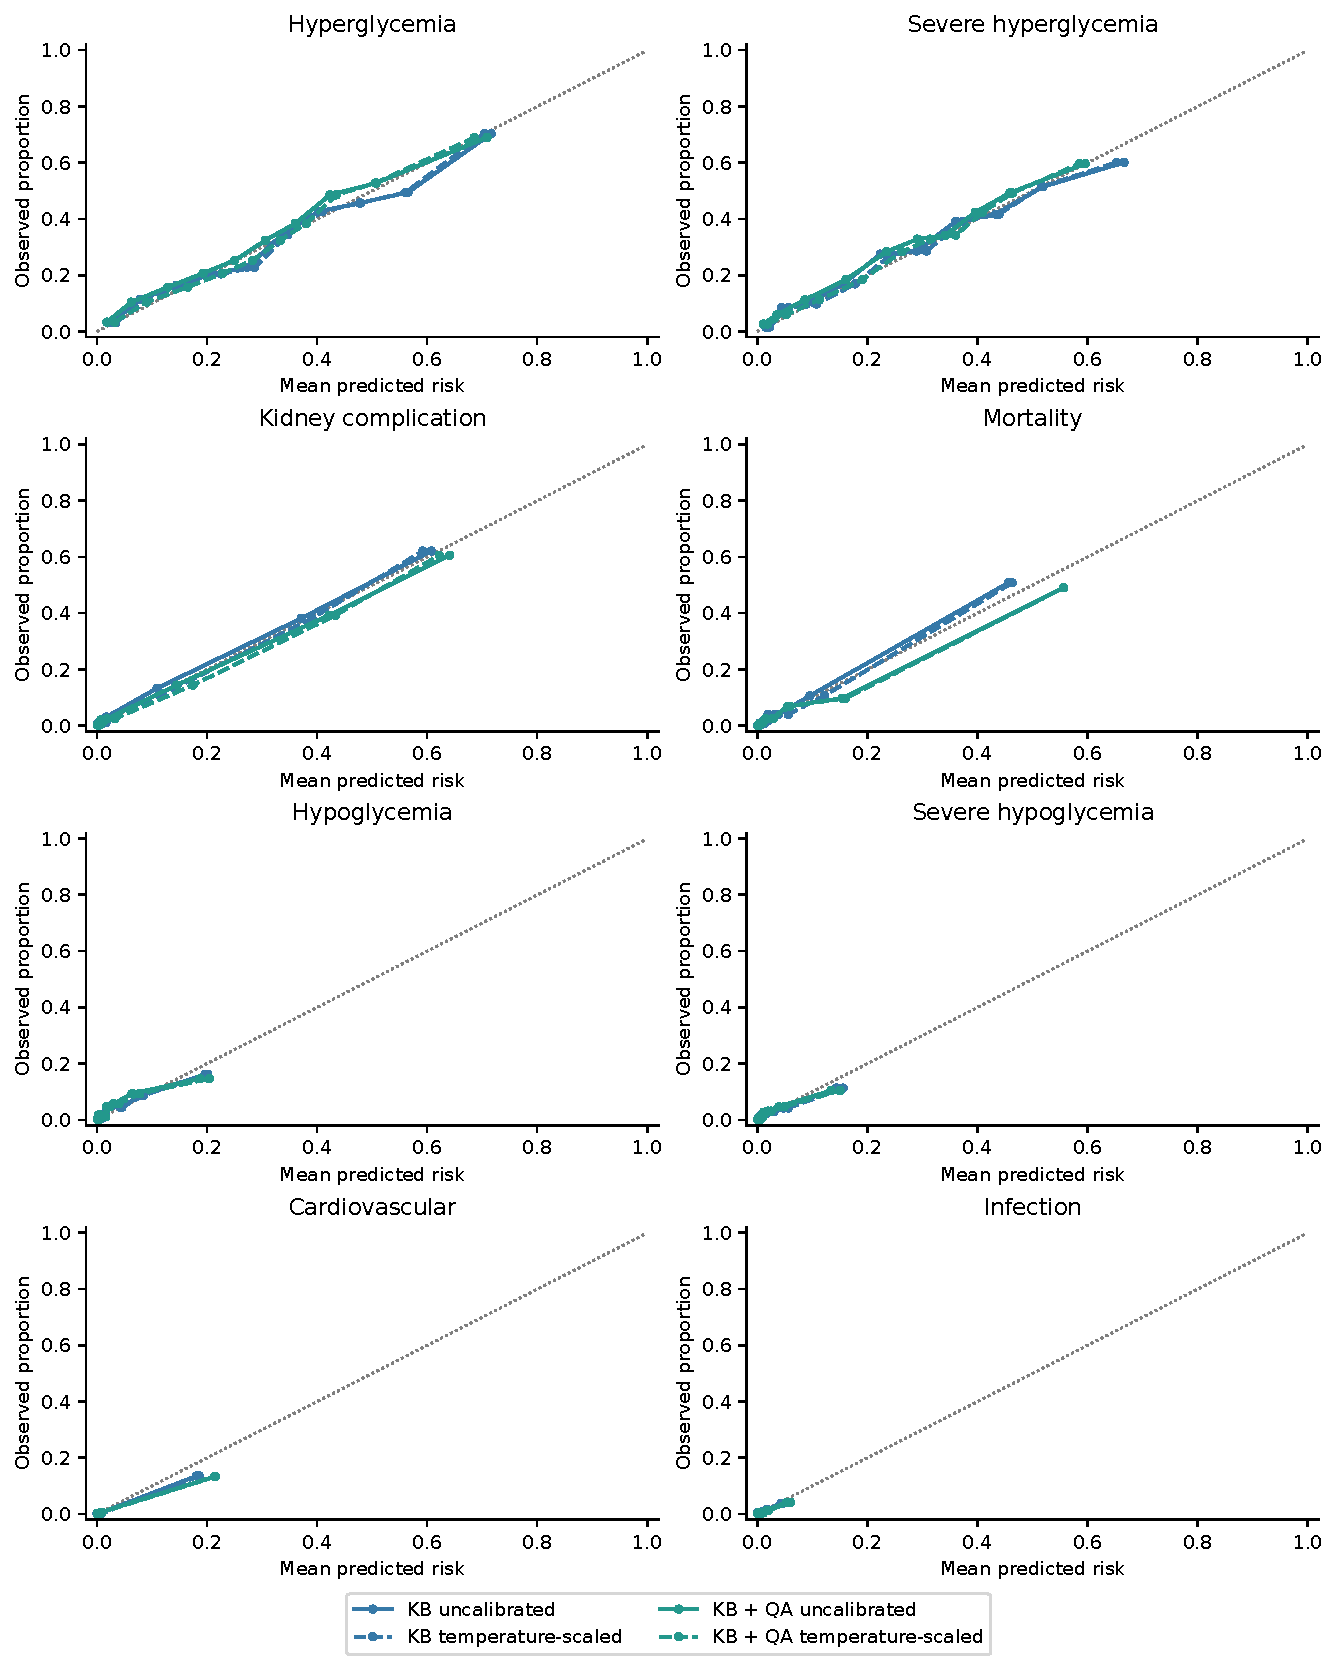
\includegraphics[width=\linewidth,height=.85\textheight,keepaspectratio]{updated_reliability}\caption{Reliability diagrams for KB and KB+QA before and after temperature scaling fitted on validation predictions. Each point compares mean predicted risk with the observed event proportion in one bin. Points on the dotted diagonal indicate agreement. Points below the line indicate overprediction, and points above it indicate underprediction.}\end{figure}
\clearpage
\section{Transcoder reconstruction and attribution to clinical concepts}
Across 300 test admissions, the largest difference in risk logits with and without the transcoders was zero. The reconstruction table gives the fraction of variation in each layer's output that the sparse features captured on validation data. Their partial reconstruction limits how fully the attributions describe each prediction. The main Discussion interprets selected associations with named clinical patterns. These exploratory findings have not been validated independently and do not estimate treatment effects.
\begin{table}[htbp]\centering\caption{Variance explained ($R^2$) and fraction of active features in each layer on held-out validation tokens.}\begin{tabular}{lrrr}
\toprule
Layer & $R^2$ & Active fraction & Validation tokens \\
\midrule
0 & 0.428 & 0.0348 & 13013 \\
1 & 0.412 & 0.0117 & 13013 \\
2 & 0.396 & 0.0343 & 13013 \\
3 & 0.514 & 0.1073 & 13013 \\
\bottomrule
\end{tabular}
\end{table}
\begin{table}[p]\centering\small
\caption{All QA concepts among the top 25 named inputs for each outcome (22 outcome--concept pairs). Ranks are based on the absolute mean contribution across admissions and include all clinical concepts. The mean score retains its sign. False and Partial are the recorded values of the assessment patterns.}
\begin{tabular}{>{\raggedright\arraybackslash}p{3.2cm}>{\raggedright\arraybackslash}p{8.3cm}rr}
\toprule
Outcome & QA concept & Rank & Mean score \\
\midrule
Hyperglycemia & Routine glucose monitoring (Partial) & 24 & -0.0127 \\
\midrule
Severe hyperglycemia & Insulin after hyperglycemia (False) & 19 & 0.0123 \\
 & Routine glucose monitoring & 23 & -0.0115 \\
\midrule
Kidney complication & Insulin after hyperglycemia (False) & 8 & -0.0317 \\
 & Routine glucose monitoring & 16 & -0.0152 \\
 & Routine basal dosage (False) & 25 & -0.0112 \\
\midrule
Mortality & Routine glucose monitoring & 14 & -0.0261 \\
\midrule
Hypoglycemia & Insulin after hyperglycemia (False) & 7 & -0.0264 \\
 & Routine basal dosage (False) & 10 & 0.0226 \\
 & Routine glucose monitoring & 12 & 0.0195 \\
 & Routine glucose monitoring (Partial) & 15 & 0.0145 \\
\midrule
Severe hypoglycemia & Insulin after hyperglycemia (False) & 7 & -0.0259 \\
 & Routine basal dosage (False) & 12 & 0.0214 \\
 & Routine glucose monitoring & 13 & 0.0175 \\
 & Routine glucose monitoring (Partial) & 18 & 0.0121 \\
\midrule
Cardiovascular & Insulin after hyperglycemia (False) & 12 & -0.0272 \\
 & Glucose monitoring on admission (Partial) & 15 & 0.0239 \\
\midrule
Infection & Routine glucose monitoring & 12 & -0.0206 \\
 & Insulin after hyperglycemia (False) & 15 & -0.0132 \\
 & Glucose monitoring on admission & 19 & -0.0073 \\
 & Routine basal dosage (False) & 20 & 0.0070 \\
 & Routine glucose monitoring (Partial) & 25 & -0.0064 \\
\bottomrule
\end{tabular}
\end{table}
\clearpage
\begin{figure}[p]\centering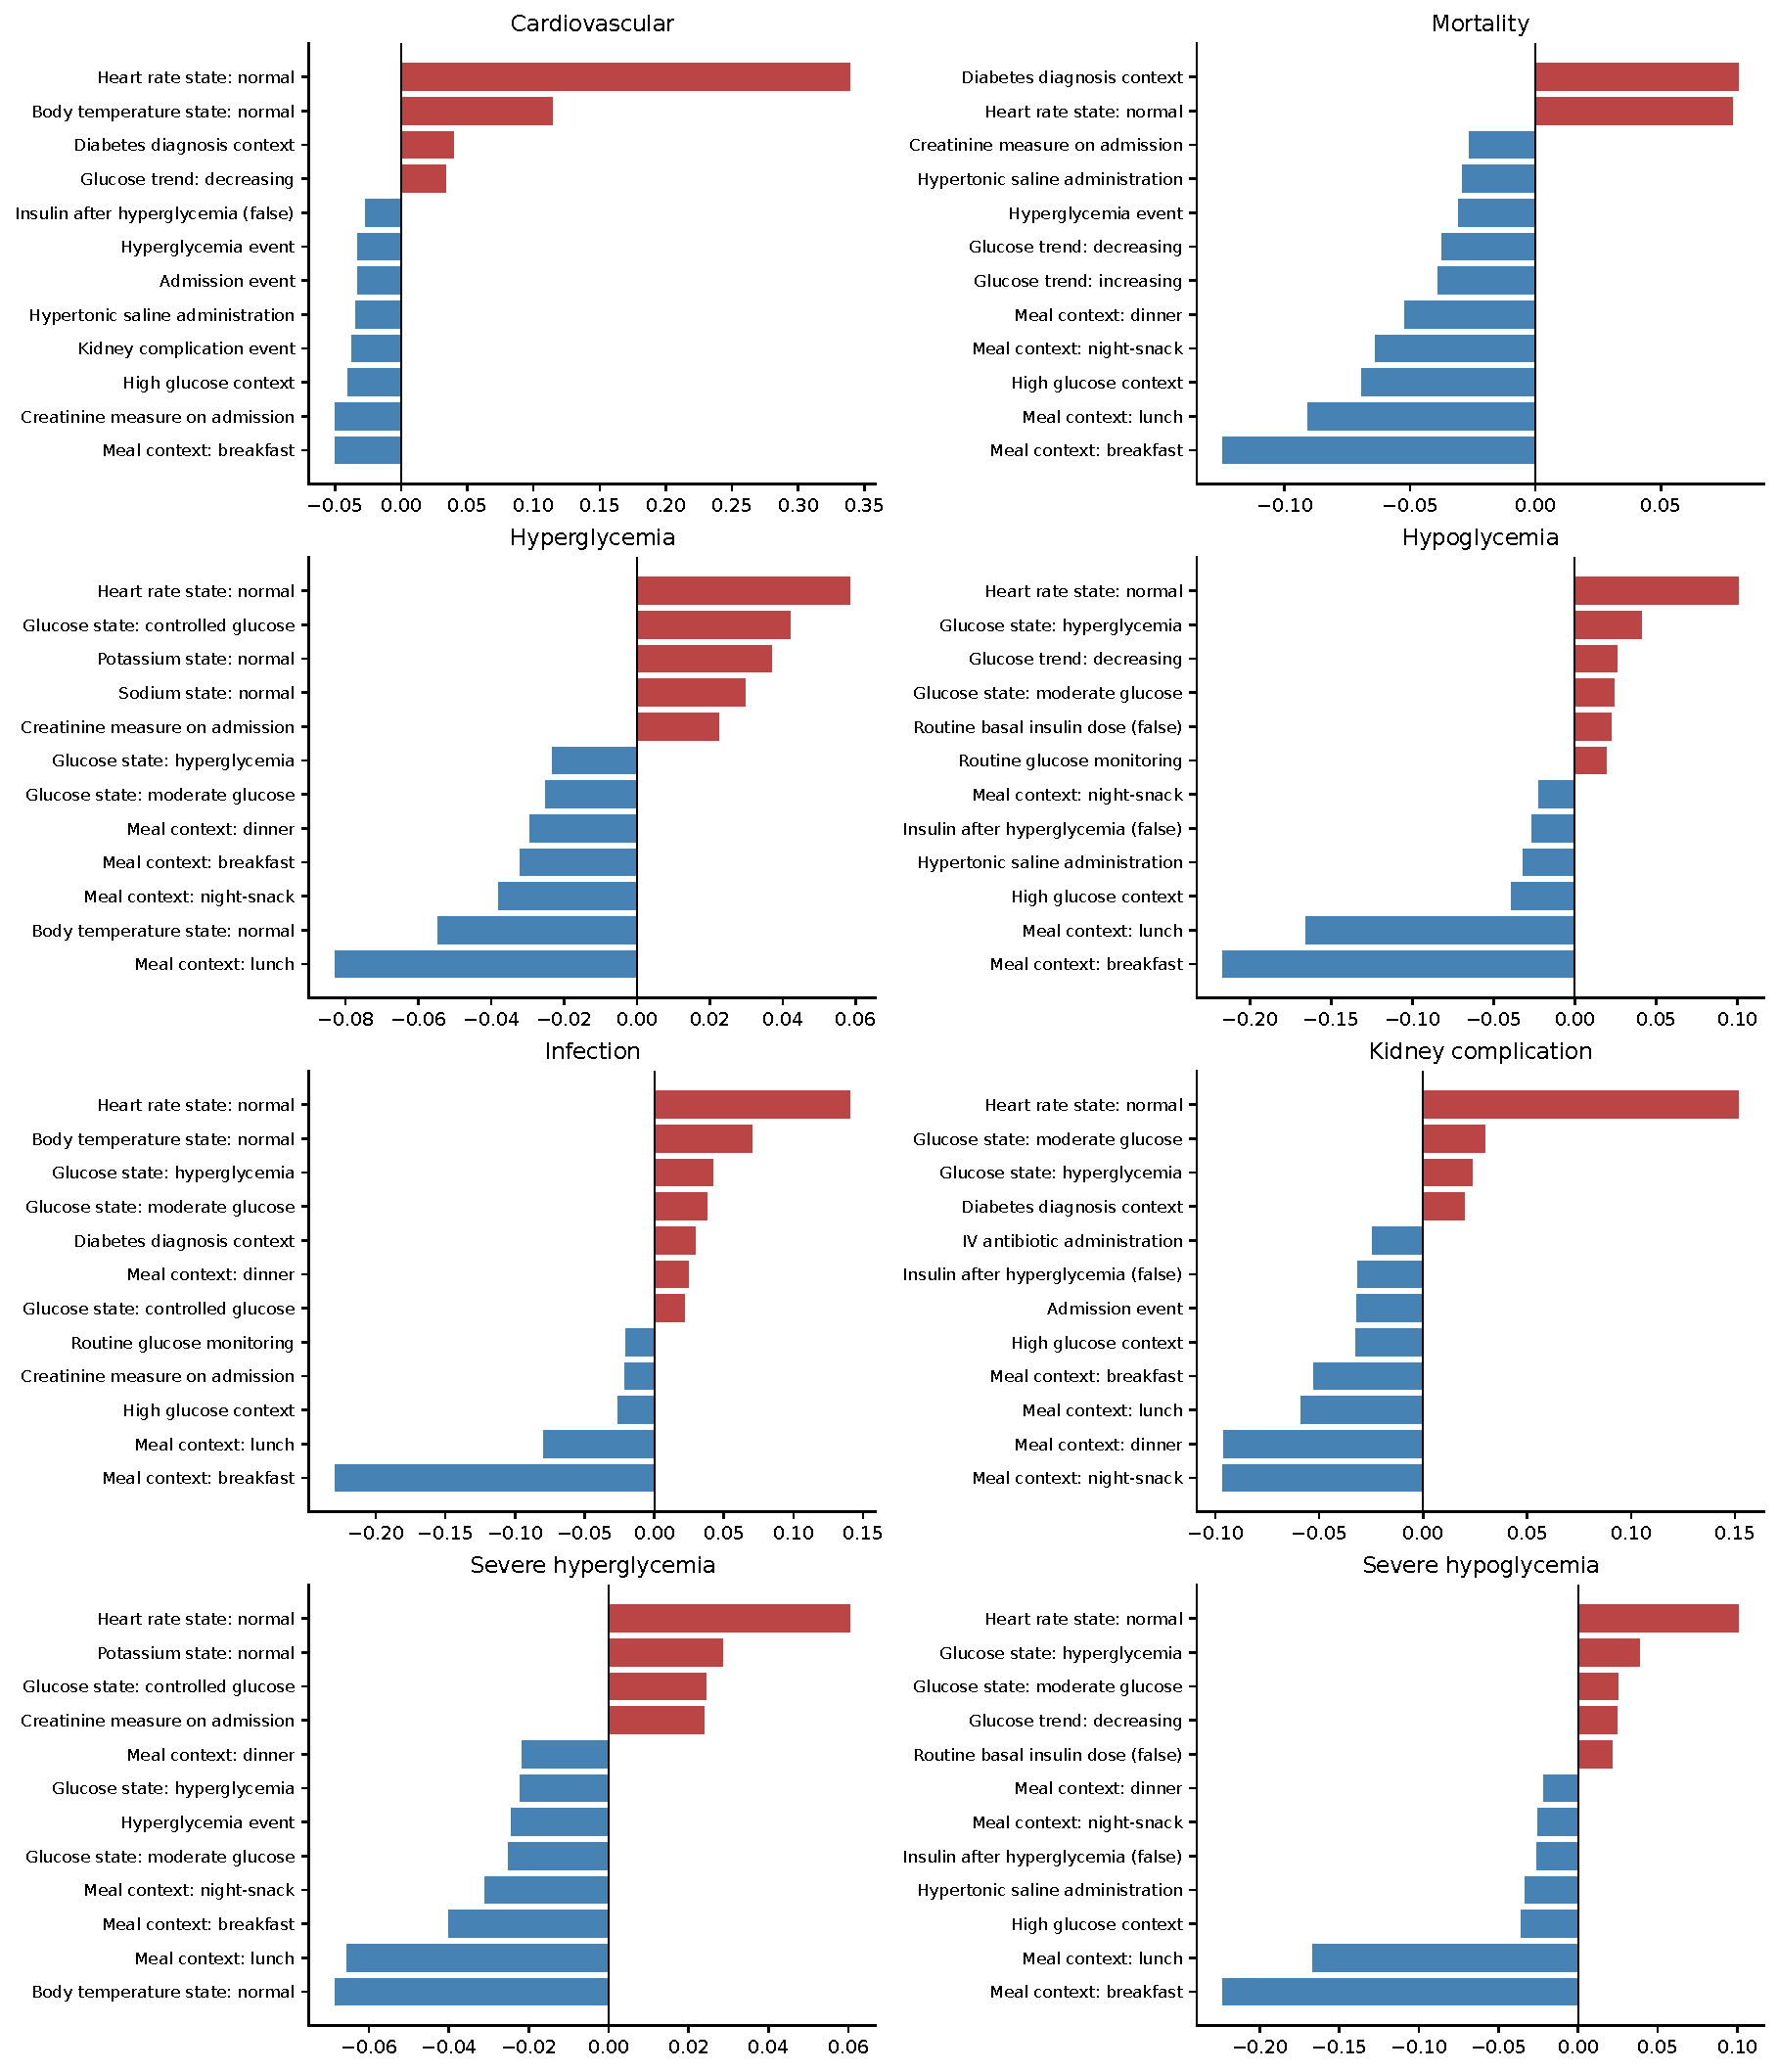
\includegraphics[width=\linewidth,height=.87\textheight,keepaspectratio]{updated_named_attribution}\caption{Signed mean contributions of selected clinical concepts in the explanation sample. Each score expresses the fitted model's sensitivity at inputs bearing that clinical name.}\end{figure}
\clearpage
\section{Distances between trained concept embeddings}
The START and END of the same concept were closest in the original embedding space (median cosine distance 0.180 across 205 pairs). For pairs sharing an abstraction, the median was 0.226 (1,500 pairs). It was 0.443 for pairs sharing only an underlying variable (1,484 pairs) and 0.590 for pairs with different underlying variables (80,656 pairs). These distances are descriptive because the same embedding can appear in several pairs.

\section{Stability of numeric states and trends}
In a sample of 500 people, we assessed 26 directly defined numeric states and their associated trends. We excluded one derived, multivariate definition. None of the perturbations added covered time in the reported state or trend summaries. The analysis evaluated the clinical intervals themselves and did not test QA patterns or downstream predictions.
\begin{table}[htbp]\centering\small\caption{Agreement in the labels assigned to covered time and proportion of baseline coverage lost. Noise is expressed relative to local threshold spacing. Intervals use 2,000 valid resamples.}\resizebox{\linewidth}{!}{\begin{tabular}{lrrr}
\toprule
Perturbation & Family & Agreement (95\% CI) & Lost coverage (95\% CI) \\
\midrule
noise\_1pct & state & 0.985 [0.984, 0.987] & 0.000 [0.000, 0.001] \\
noise\_1pct & trend & 0.996 [0.995, 0.997] & 0.000 [0.000, 0.001] \\
noise\_5pct & state & 0.976 [0.975, 0.978] & 0.001 [0.001, 0.002] \\
noise\_5pct & trend & 0.980 [0.978, 0.982] & 0.002 [0.001, 0.003] \\
remove\_10pct & state & 0.974 [0.973, 0.976] & 0.020 [0.018, 0.021] \\
remove\_10pct & trend & 0.953 [0.950, 0.956] & 0.032 [0.029, 0.034] \\
remove\_5pct & state & 0.989 [0.988, 0.989] & 0.008 [0.008, 0.009] \\
remove\_5pct & trend & 0.977 [0.975, 0.979] & 0.015 [0.013, 0.016] \\
\bottomrule
\end{tabular}
}\end{table}
\clearpage
\section{Timing predictions from training medians}
\begin{table}[htbp]\centering\small
\caption{Day-four timing baselines in hours. Each prediction is a median estimated in training, measured from admission. Onset errors use only admissions with the outcome in the forecast window. Mortality timing refers to the death-coded visit end. Confidence intervals use 2,000 bootstrap samples clustered by person.}
\label{tab:s-medians}
\begin{tabular}{lrrrr}
\toprule
Outcome & Training $n$ & Test $n$ & Prediction (h) & Test MAE (95\% CI, h) \\
\midrule
Cardiovascular complication & 341 & 66 & 130.54 & 39.66 [28.56, 52.11] \\
Mortality & 1,628 & 329 & 182.95 & 57.87 [54.08, 61.97] \\
Hyperglycemia & 6,556 & 1,427 & 127.30 & 27.65 [26.23, 29.20] \\
Hypoglycemia & 728 & 178 & 136.13 & 38.52 [33.47, 44.11] \\
Infection & 208 & 33 & 135.56 & 24.92 [16.52, 35.34] \\
Kidney complication & 2,324 & 545 & 136.48 & 33.56 [30.50, 36.76] \\
Severe hyperglycemia & 5,899 & 1,285 & 125.80 & 28.07 [26.55, 29.61] \\
Severe hypoglycemia & 491 & 108 & 139.37 & 42.89 [36.36, 50.17] \\
\midrule
Length of stay & 20,994 & 4,508 & 152.28 & 48.47 [47.33, 49.75] \\
\bottomrule
\end{tabular}
\end{table}
\clearpage
\section*{Supplementary Methods A. Regression features and model size}
One row represented one admission at one observation cutoff. We used eligible raw observations from admission through that cutoff, in time order. Numeric observations retained their values, and true and false were encoded as one and zero. Each remaining categorical concept--value combination became a separate indicator variable with value one at each occurrence. We kept variables observed in at least 2\% of training admission--cutoff pairs and used the training feature columns for validation and testing.

For each retained variable, the vector contained 14 summaries. Ten described the values and their frequency, namely count, mean, sample standard deviation, minimum, maximum, 25th percentile, median, 75th percentile, first value, and last value. Four described the observation history, namely an indicator of any observation, hours between the first and last observations, change from first to last divided by that span in hours, and count divided by the span in days. For a zero span the slope was zero. For the rate, the denominator was bounded below at $10^{-6}$ days.

When a variable was absent, its observation indicator, count, span, and rate were zero. We joined these features to the admission-level covariates, including elapsed observation time and remaining forecast time. For each guideline pattern, the QA variant included its mean score (zero when no score was available) and a binary indicator of any assessment completed by the cutoff. For other missing entries, we used the training-column median, with zero as the fallback for an entirely missing column. Each column with missing entries in training received a separate missingness indicator. We aligned validation and test columns to the training matrix, filling absent columns with zero, then standardized all columns using training means and standard deviations, using a divisor of one for constant columns.

The 13 pattern means and 13 occurrence indicators added 26 features to the 1,510-feature regression vector, giving 1,536 inputs with QA. The clinical study reported 14 scored components because it assessed routine basal insulin dosage for both administration frequency and dose amount. Both assessments carry the same pattern name. The vector therefore pooled the two aspects under one pattern name, giving 13 named patterns across the 14 components \citep{oded2027kineret-jbi}. The eight risk estimates, eight onset estimates, and length-of-stay estimate each used a linear function of the same vector, with a logistic link for risk. With 17 intercepts, these dimensions give 25,687 coefficients without QA and 26,129 with QA. 

The supervised STraTS comparators used two layers, 16 attention heads per layer, and a hidden dimension of 64 (91,441 parameters without QA). Each of the 26 added inputs connects to 128 units in the context projection, giving 94,769 parameters with QA. The four-layer clinical interval encoder had approximately 1.68 million parameters before the supervised prediction heads were attached. For KB+QA, the rounded encoder count for the score inputs was 1.69 million, and the 13 occurrence indicators add 1,664 weights to its context projection. The supervised attention pool and prediction heads added 166,786 parameters to each encoder. Together these dimensions give approximately 1.85 and 1.86 million parameters for the full KB and KB+QA models. SAX used the same encoder dimensions with a different input vocabulary. Its fitted encoder contained 1,734,152 parameters, giving 1,900,938 with the prediction heads.

We retained the encoder width of 128 and two attention heads per layer used in the earlier ICU study. In that study, an encoder with width 64 and one head per layer (0.46 million parameters) also exceeded ss-STraTS on AUPRC (0.646 versus 0.627) \citep{oded2026intervene}. For ss-STraTS we retained the published architecture with the width, layer count, and attention head count used in our earlier comparison. For a sensitivity analysis, we increased the hidden width of ss-STraTS from 64 to 304, bringing its parameter count close to that of KB. Both ss-STraTS runs used the same inputs without QA, two layers, 16 heads, the same training settings and seed, and the same validation rule for selecting the checkpoint. We evaluated all three models on the same 4,508 day-four test admissions. The learning rate and dropout were those used for the default width. Under this fixed protocol, the wider model had lower discrimination on each summary measure (Table~\ref{tab:s-width}).

\begin{table}[htbp]\centering\small
\caption{Discrimination at day four in the ss-STraTS width sensitivity analysis. Paired differences use the first model minus the second. The 95\% intervals use 2,000 valid bootstrap samples clustered by person and describe uncertainty in the test population for the fitted models.}
\label{tab:s-width}
\begin{tabular}{lrrrr}
\toprule
Model & Parameters & Weighted AUPRC & Macro AUPRC & Weighted AUROC \\
\midrule
ss-STraTS (64) & 91,441 & 0.4747 & 0.3704 & 0.7701 \\
ss-STraTS (304) & 1,825,909 & 0.3950 & 0.3079 & 0.6886 \\
INTERVenE KB & $\approx$1.85M & 0.5274 & 0.4024 & 0.8033 \\
\bottomrule
\end{tabular}

\smallskip
\begin{tabular}{lrr}
\toprule
Paired difference & Weighted AUPRC (95\% CI) & Weighted AUROC (95\% CI) \\
\midrule
KB minus ss-STraTS (304) & $0.1323\ [0.1128, 0.1531]$ & $0.1147\ [0.1011, 0.1284]$ \\
ss-STraTS (304) minus (64) & $-0.0796\ [-0.0945, -0.0652]$ & $-0.0816\ [-0.0923, -0.0703]$ \\
\bottomrule
\end{tabular}
\end{table}

\clearpage
\section*{Supplementary Methods B. From glucose readings to interval tokens}
The open Temporal Mediator implementation by Shahar Oded includes the diabetes knowledge base used in this study \citep{mediator-github}. Separate rules use the glucose readings to derive a state and a trend \citep{shahar1997framework,oded2026intervene}. A reading of 210 mg/dL falls in the hyperglycemic band. Consecutive readings in that band can form a state interval under the persistence rule. The glucose trend rule fits a slope to readings in the trailing 12 hours. A fitted change of at least 40 mg/dL over that window in either direction gives an increasing or decreasing trend. Smaller changes, or an insufficient history to estimate a slope, give a steady label. The trend extends from the current reading to the next only if the gap is at most 24 hours. Adjacent intervals with the same trend are merged. Thus a glucose state can remain high during a decreasing trend.

Figure~\ref{fig:s-boundaries} shows how each boundary records its time and four identities. The start and end of a high-glucose interval share the raw concept (glucose), abstraction (state), and value (high). Only the boundary identity changes. Over these clinical histories, the Mediator also recognizes quality-assessment temporal patterns, such as insulin administration after hyperglycemia. The KB+QA model can read the dated assessments alongside the states and trends.
\begin{figure}[htbp]\centering
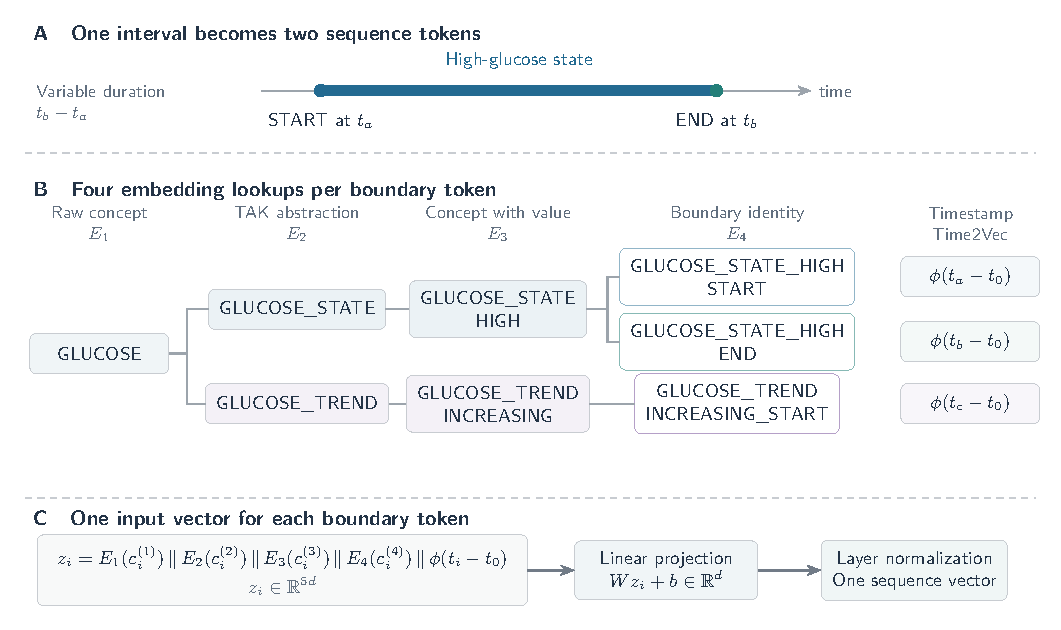
\includegraphics[width=.83\linewidth]{intervene_hierarchy_tokenization}
\caption{Boundary identities and timing for a high-glucose interval. Reproduced from the INTERVenE methodological study \citep{oded2026intervene}.}
\label{fig:s-boundaries}
\end{figure}
\small
\setlength{\bibsep}{3pt}
\bibliographystyle{elsarticle-num}
\bibliography{references}
\end{document}

